\section{Analysis}
\label{sec:analysis}


    Name squatting in Namecoin has been previously discussed as an issue facing the cryptocurrency. There have been several solutions proposed to alleviate the squatting issue by implementing new protocols or by placing additional fees on certain actions to either deter the actions of squatters or make it possible for a legitimate user to acquisition a desired name from a squatter if it increases the economic use of said name. In this section, we analyze some of the more popular methods, and discuss the costs to various individuals for each. 
    As it exists now, the only cost for an individual to register a name is the 0.01 NMC used to make the token, and then 0.01 NMC to cover two transactions fees (0.005 NMC each), one for the NAME\_NEW and one for the NAME\_FIRSTUPDATE transaction. Holding onto a name bares almost no cost with the owner only needing to pay 0.005 NMC as a transaction fee every time they post a NAME\_UPDATE transaction (which they need to do about once every 250 days). Losing a name doesn't cost a user anything, and the user gets gets the 0.01 NMC token back as a normal coin. 

\subsection{Adding a Cost to Updating Names}
    One of the most commonly suggested, and simplest, solutions to squatting is to add an associated fee with updating a name. The idea is that such a fee will not hinder a legitimate user very much, but will cause a squatter holding onto many domains to have to pay enough for the squatting to become financially infeasible. The reason that such a feature hasn't been implemented is because the Namecoin developers fear that the increased fees will disincentivise Namecoin adoption. Additionally, of the current squatters, some are benevolent and will give away names to users who have legitimate uses for the domains. Adding the renewal fees would punish these users who do not stand to gain monetarily from their efforts. This approach is very strong when it comes to deterring squatters who register thousands of domains. It is less effective against the type of squatter who registers just a few names that they think will be particularly valuable (like google.bit or poker.bit), or the type of squatter who is trying to squat on a name without the intent to sell, but just to hurt who they think the name would be valuable to.
For our analysis, we look into an update fee of 0.1 NMC. In this scenario, every time a user creates a NAME\_UPDATE transaction, a domain owner must burn 0.1 NMC for the transaction to be valid. Adding this fee wouldn't change the initial cost of registration, it would still be 0.02 NMC (0.01 from creating the token, and 2 transaction fees). The update fee will, however, change a user's cost on an update from 0.005 NMC to 0.105 NMC. Once the name expires, the user will again recoup their 0.01 NMC token that they attached to the name. 

\subsection{Varying Registration Costs Based on Name Lengths}
    Another commonly suggested solution is to vary the registration cost based on the length of the name. Shorter names are easier to remember, so the idea is they are generally worth more in practice and should cost more when they are registered. There have been various schemes suggested for the specifics on how the price should scale with name length, most of which resulting in exponentially decreasing costs for longer names. One issue with this approach is that the implicit assumption of this model, that shorter names are more valuable, may or may not actually reflect reality. Our results show that in the d/ namespace, more shorter names are taken, but this doesn't necessarily mean that they are more valuable. We speculate that a name like amazon.bit is probably more valuable than xyz.bit, and this wouldn't be reflected with this kind of pricing scheme.  This method does provide a good deterrent against squatters who are trying to claim many short names, but is rather ineffective against a squatter who is either trying to claim specific, valuable domain names, or hoard large quantities of longer domain names. 
    There exist many pricing protocols, but we have chosen to analyze the strategy outlined on the Namecoin Pricing wiki in more depth. According to this system, the prices depended on multipliers of an arbitrary price for different name lengths. 

\begin{figure*}
  \centering
  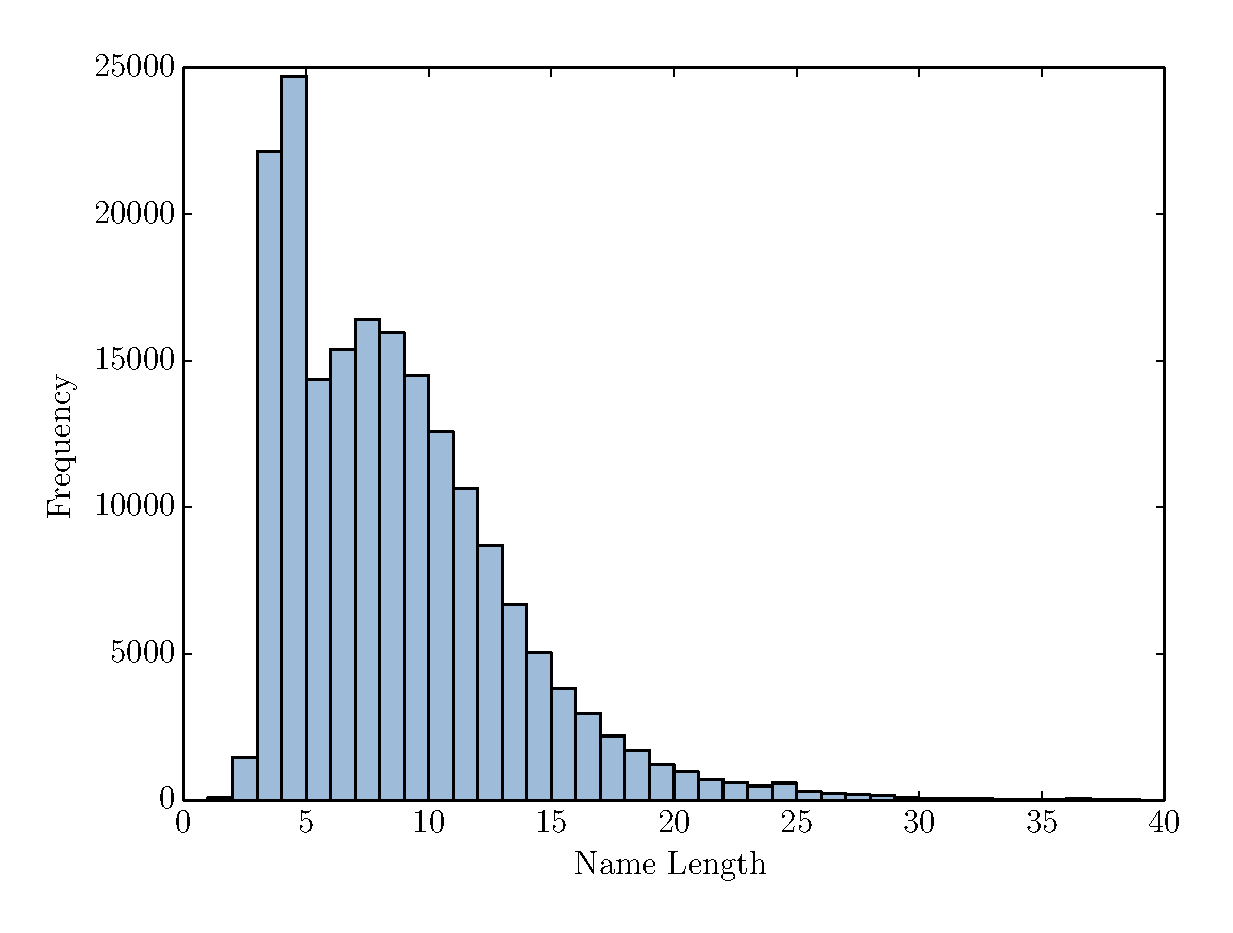
\includegraphics[width=0.95\textwidth]{figures/name_length_histogram}
  \caption{Length of Registered Names}
  \label{fig:nameLength}
\end{figure*}

\begin{table}[t]
  \centering
    \rowcolors{1}{}{lightgray}
  \begin{tabular}{| l | l |} \hline
    Length in Characters & Cost Multiplier \\
    1-3 & \( 5 x \) \\
    4-6 & \( 2 x \) \\
    7-14 & \( 1 x \) \\
    15-20 & \( \frac{1}{2} x \) \\
    21 + & minimum cost \\ \hline
  \end{tabular}
  \caption{Length based multipliers.}
\end{table}




    We use 0.5 NMC (could change) as the arbitrary price to be multiplied for our cost estimations. The update fees and the returned token are the same in this method as they are in the existing structure. The only change in cost is in the registration fee. In order to calculate what an average name would cost to register under this protocol, we have uniformly taken random names from the distribution of name length, and averaged the registration cost of these names. 



\subsection{Auctions}
    In this method for dealing with squatters, the Namecoin protocol could enforce that domain names are put up for auction on a periodic basis (perhaps every 52,000 blocks or about once/year). The protocol would allow for an auction after enough time has passed since the last auction, or since the NAME\_FIRSTUPDATE transaction for any given name. When an auction occurs, a name will become available and whomever is willing to pay the most for the domain name will get the name. In order to make it easier to retain a name, it has been suggested that the current owner should get some sort of advantage in the auction, so that the only need to bid some fraction of the highest bid in order to retain the name (let this be 1/100 for this discussion). If the current owner wins the auction, then they 'pay the network'. The cleanest way to do this is to burn the coins. Essentially, if the market cap of the currency doesn't change, then burning the coins from the auctions would uniformly increase the value of all the other remaining coins (burning too many coins can cause its own problems, too. Paying the network could also be done through other means, such as paying a random active address in the blockchain). The overall result should be that the fee paid for retaining a name should be spread out amongst other users of system. If, on the other hand, a new user wins the auction and bids more that 100 times the bid of the current owner of the name, the new user will gain the name, and the old owner will be the recipient of the auction coins. 
    An auction system like this has many disadvantages. The largest issue with this kind of squatting solution is that it erodes .bit's resistance to anti-censorship. One of the fundamental ideals of Namecoin and the .bit TLD is that it promotes freedom of speech, where a central authority is unable to censor content. Allowing a party to claim a domain as long as they are willing to pay enough undermines this concept. Periodic auctions would allow any large entity, such as an oppressive government, to easily seize names from any smaller entity that they want to silence. The counter argument here is that if a large entity seizes a smaller entities domain, the small entity would get paid a considerable sum-- in this case, 100 times what they were willing to bid to keep the domain. Whether or not the cash received by the censoring of the domain is worth more to the small entity than having the domain is a question that we do not explore.  An additional weakness of this system is that it can cause a legitimate user to have to pay lots of money in order to keep their domain every auction. Even with a large advantage, if owning a particular .bit domain is of great importance to an individual, then they can be forced to pay a large sum of money every auction. If "Business" is trying to hold onto business.bit, and business.bit is worth a considerable amount to them (say they get many online sales there), then a competitor to Business could bid some factor  less than what business.bit is worth to Business. Business isn't willing to part with business.bit for this amount of money, so they are forced to instead pay 1\% of what business.bit is worth every time there is an auction for their domain.
    Under this model, the initial cost a domain depends on how an individual acquires the domain. If they acquire the domain without an auction, then the cost is the same as it is in the existing protocol. Conversely, if an entity acquires a domain through the auction process, then the fee they will need to pay will depend on the value of the domain to whomever they are buying it from. If the seller is a squatter, the buyer will need to bid an amount equal to what the squatter thinks the domain is worth (the squatter will bid 1\% of what they think the domain is worth). Holding onto a domain in this model can be expensive; as discussed previously, every time there is an auction, the owner of a domain can be forced into paying 1\% of what the domain is worth to them, which could be a sizeable amount of money. Aside from the auction costs, there is still the small transaction fee that the owner will need to pay for every NAME\_UPDATE transaction. If a user lets their name expire, this situation is identical to the ones previously discussed, but if an individual loses control of a name because of an auction, they don't get their 0.01 NMC token back and they instead get the money from the auction. In this case, they receive an amount of money equal to the value of the domain to them. 

\subsection{Require an Escrow}
    Another proposed solution is to require a number of namecoins to be put into an escrow account when claiming a name. The money in escrow would be locked, so that the owner of the name is unable to spend that money, but once the owner loses or forfeits the name, the money in escrow is returned. The exact amount of money to be put into escrow is a debated topic. In one such model, the amount is decided by the owner of the name. In this situation, there would be an additional protocol designed to allow someone to take a name if they are willing to pay more money into an escrow account for said name than the current owner. If someone tries to place more money into escrow than the current owner (in an attempt to take the name), the current owner is notified and has a short grace period in which they can protect themselves by placing a larger amount of money in the escrow account. In order to prevent the the same problems and censorship erosion as seen in the case with auctions, there is a maximum allowed escrow and once a domain owner fills the escrow to this amount, the name becomes locked and it would be impossible for another user to seize for any amount of money (let this maximum value be 200 NMC). This provides reasonable financial protection against squatters who are trying to squat on thousands of domains, because a squatter such as this would need to fill the escrows for any of the domains that they are squatting that other people want. If a user out-escrows a squatter, this represents an ultimate failure in the eyes of the squatter because they lose the domain name and get paid nothing. The only way for a squatter to prevent this is to continue to fill their escrows for names that a user wants until the escrows are full. Once the squatter puts money into escrow, they can't remove it without losing the name, so eventually all of the escrows for all of the names users want would need to be full. This penalizes certain squatters more than others, in the sense that the squatter will always eventually get their coins back. A squatter that doesn't need access to their coins has no issue with locking up some huge fraction of them in escrow, because they will eventually get the coins back. A poorer squatter, on the other hand, who doesn't have enough coins to have some of them locked up for every domain they try to squat, will be forced to stop. 
    The cost of registering a name is now variable because a user can decide how much or little money they want to put into escrow. This has the advantage of being acceptable to many different types of users. A serious user who is only interested in having a few valued domains and doesn't want to risk losing their domains can easily pay to fill an escrow account for their domains. At the same time, a more casual user, who just wants some domain (but not a valuable domain) can still attain this domain while only owning a small number of coins. The cost of holding onto a domain is the same as it is in the present situation. Once a domain name is lost, a user will gain access to all the money locked into escrow for that name.     

\subsection{Cost Analysis}
    In order to compare the overall costs of the various models, we consider applying the cost assumptions outlined above to different users trying to hold onto domains for a period of 3 years. One user is a squatter who is trying to hold on to 1000 domains of variable length and value. Another is a squatter who is only trying to squat 5 particularly valuable names. The final two a legitimate users, one of which is looking to use a very specific, valued domain name, and the other is a user that just wants a domain, but doesn't really care what the domain is.


\begin{table*}[t]
  \centering
  \rowcolors{3}{}{lightgray}
  \begin{tabularx}{\linewidth}{| X | X | X | X | X |} \hline
    &  Squatter with 1000 domains & Squatter with a few valuable domains & User who wants any domain & User who wants a specific, valuable domain\\
\hline
    \multicolumn{5}{|c|}{\textbf{Registration Cost}} \\ \hline
Current System &  20 NMC & 0.1 NMC & 0.02 NMC & 0.02 NMC, or best offer from squatter \\
Increasing Update fee & 20 NMC & 0.1 NMC & 0.1 NMC & 0.02 NMC \\
Length based fees & 737.77 & 3.68 & 0.74 & 0.74 \\ 
Auctions & 20 NMC & 0.1 NMC & 0.1 NMC & Fee paid in Auction \\
Escrow & 200,000 NMC & 1,000 NMC & 0.02 NMC & 200 NMC \\ \hline

\multicolumn{5}{|c|}{\textbf{Longer term cost (3 years of Updates)}} \\ \hline
Current & 25 NMC & 0.125 NMC & 0.025 NMC & 0.025 NMC \\ 
Increasing Update fee & 500 NMC & 2.5 NMC & 0.5 NMC & 0.5 NMC \\ 
Length based fees & 25 NMC & 0.125 NMC & 0.025 NMC & 0.025 NMC \\ 
Auctions & & & 1 \% of what domain is worth to user & 1 \% of what domain is worth to user \\ 
Escrow & 25 NMC & 0.125 NMC & 0.025 NMC & 0.025 NMC \\ \hline

\multicolumn{5}{|c|}{\textbf{Refund Upon Losing Name}} \\ \hline
Current & 10 NMC & 0.05 NMC & 0.01 NMC & 0.01 NMC \\
Increasing Update fee & 10 NMC & n0.05 NMC & 0.01 NMC & 0.01 NMC \\
Length based fees & 10 NMC & 0.05 NMC & 0.01 NMC & 0.01 NMC \\
Auctions & & & What the domain is worth to user & What the domain is worth to user \\ \hline
  \end{tabularx}
  \caption{Cost comparison of the various anti-squatter mechanisms.}
\end{table*}


\subsection{Analysis of OneName}
    Analyzing the names on the blockchain reveals that the online identity service, OneName, holds a very large user base. After identifying and removing probable squatters, using the strategies listed in Methods, OneName has roughly 20,000 unique names/values, which dwarfs the 1000 or so unique name/values in the d/ namespace. This provides evidence that Namecoin can be more successfully used for applications other than a domain name look-up service. The idea behind OneName is that a user can have a name/value pair in the blockchain that associates said name with different online identities such as an email, GitHub, or Twitter. If it is verified that these accounts are owned by the same person who owns the name/value pair (generally by posting a message with each of their accounts with a specific string mentioning the OneName name in the blockchain), then others can trust that a single entity owns all these accounts. 

We think there are several reasons why OneName has become more popular than d/, the most significant of which being that OneName completely abstracts away the involvement of Namecoin. In order to make a OneName identity, a user only has to visit OneName's website to create an account. OneName takes the information given to it and puts it into a name/value pair and posts that into the Namecoin blockchain. The user doesn't need to know anything about Namecoin, have Namecoins, or even know that Namecoin is working behind the scenes in order to complete the process. One reason this model works for OneName is because name/value pairs have become quite cheap. Registering a name only costs 0.01 NMC for the token and 0.01 NMC to cover two transactions fees. It then only costs 0.005 NMC every 250 days or so to update the name/values to keep them fresh. Given the current exchange rate of Namecoin to dollars, this represents a cost of approximately one cent for OneName to post one of its user's information into the blockchain. Even with a user base as large as 20,000, OneName's expenses to cover everyone's fees total to only a few hundred dollars. OneName has made the assumption that picking up the tab on the fees is well worth sparing their users the effort of trying to use Namecoin, and it seems that this approach is successful.

This leads to our next point; it isn't the cost that prevents people from registering name/values in the Namecoin blockchain, it's the inconvenience. A user who has no Namecoins to begin with is faced with large hurdles in order to register a name. The first step is acquiring a Namecoin client. While not particularly difficult to install, the standard Namecoin client requires the user to become a Namecoin node which means they will have to download, verify, and store the entire blockchain. The next obstacle for a user is to acquire coins. This is more tricky than it appears because no exchange will sell cryptocurrencies like Namecoin or Bitcoin to users who use credit cards. This is impossible for exchanges because users can challenge the charges on their card, and the exchange can't easily provide proof that they sent the coins to an address the user controls. Assuming the user has Bitcoins, or is willing to buy Bitcoins (which still has to be done without a credit card-- it could be done in person or, more commonly, the user could use Coinbase and hook a Bitcoin wallet up to their bank account), then the user will need to convert these coins to Namecoin. Many exchanges will do this, but it isn't particularly pleasant. In our experience, after making an account, the exchange required us to wait for three days before we were allowed to convert our Bitcoins to Namecoins. At this point, the user is finally ready to start making the NAME transactions outlined in the registration protocol section. They must then either remember to update their names every 250 days, or use some software that will automatically take care of updates.

This leads to an interesting question: if using Namecoins is so inconvenient that it deters potential adopters, then why does the actual system require users to pay? Most of the miners are merge mining, and the majority of their Namecoins come from the block reward, so why require a transaction fee on NAME transactions? The reason these transactions need to have associated fees is to stop squatters. Squatting is already a major issue, but it would be much worse if claiming a name was free. As it is now, if a squatter wants to register a few thousand names (as many of them do),  it represents a reasonable investment from the squatter. If the squatter has to invest a few hundred dollars, then they must feel that they can potentially earn this money back from selling some of the domains they squatted. If it costs nothing to claim a name, then the investment from the squatter is nothing, and even if they only sell one of their millions of squatted domains, then they will profit. 

The next logical step is that, because it is free, OneName should suffer from a massive number of squatters. According to the data in the blockchain, however, this is simply not true. OneName actually has a much better user to squatter ratio with only a few thousand squatters on on their namespace (including OneName itself which has also benevolently squatted some of the names in its domain space to save usernames for well known individuals). This is a result of a few different factors. The first factor contributing to this is that in order to make the name/value pairs for free, an individual needs to go through OneName. This allows OneName to implement their own anti-squatting techniques to try to prevent a single user from claiming many usernames. Additionally, because a user goes through OneName, OneName actually owns the Namecoin address that holds the token with their data. If a squatter was to squat a valuable name, they would be unable to sell it to a buyer because OneName owns it. Even if a squatter isn't intimidated by the small fee and they try to squat through the Namecoin client, squatting OneName usernames is less valuable than squatting domains in d/. A certain name in the OneName namespace is not particularly valuable because a user doesn't really need a specific name. If John Smith is using OneName, jsmith would be a pretty ideal username, but he could just as easily use jsmith1 or jsmith912. With any of these usernames, when someone searches "John Smith" in OneName, his identity will come up. This is because OneName stores an individual's actual name in the value portion of the name/value pair, and this is how most people will search for them (unlike a domain name). The name associated with this value in the blockchain is mostly just aesthetic. Finally, a squatter would be hard pressed to find buyers in this namespace. For domain names, if a user sees that a name they want is taken, they can look at the value stored on the blockchain, see that it has a squatters contact information, and contact the squatter. As discussed previously, OneName users are insulated from the Namecoin network. They would be trying to make a new account on the OneName website which would simply tell them that a particular username is taken. Even if they are willing to pay for it, they wouldn't know who to contact without having to directly engage with Namecoin themselves. 

Another final interesting fact derived from OneName's success indicates how users value the distributed cryptographic security of their information compared to the simplicity of a service. Because OneName owns all of the name/value pairs, and the users typically never validate what OneName tells them with the blockchain, the users are completely trusting it as a central authority which leaves them vulnerable. Most users find this acceptable because even though they aren't checking the Namecoin blockchain, they know that someone could be checking the Namecoin blockchain. As long as there is the potential for someone to verify the information with the blockchain, OneName can't lie without being caught. Judging by the success of OneName, users find this pseudo security to be a close enough approximation to that provided by the Namecoin blockchain if it allows them to ignore having to deal with the Namecoin protocol. 

